\section{Approach}
Our approach to investigating the architecture for deep learning recommendation systems, was to first decide on a baseline with which we could compare the effectiveness of our techniques. After finding a benchmark we reviewed the literature we had assembled to decide which design was most applicable to our dataset, and our ability to implement.

 We knew from the Netflix competition that the winners had an RMSE of 0.8567. We also wanted a way to compare our engineered solution, to one that simple took all the data Netflix provided and used it as inputs on a naive feed-forward neural net. 

 \begin{figure}[h]
    \centering
    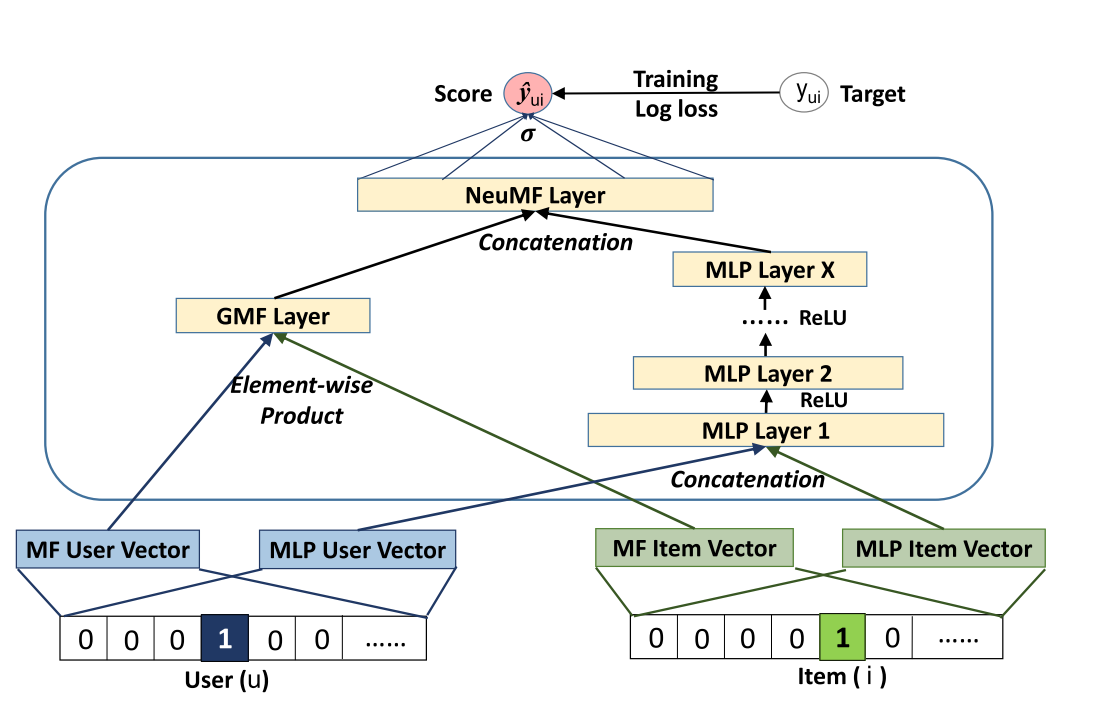
\includegraphics[width=0.45\textwidth]{images/NCF_diagram.png}
    \caption{NCF diagram}
    \label{fig:NCF diagram}
\end{figure}

 The theme of all the papers we read covering the various methodologies for applying deep learning to recommendation systems, was creating more meaningful representations of the users, the items they interacted with, and context around the item. Many of the models we read about involved many complex hierarchical layers. While many of these exotic arrangements made sense, we were not sure we had the technical expertise to implement them in the allotted time. We settled on a technique called Neural Collaborative Filtering \cite{He2017}. Neural Collaborative Filtering or NCF is a process that involves creating a hybrid of traditional recommendation system and deep learning. As you can see from figure~\ref{fig:NCF diagram} it combines user vectors and item vectors from matrix factorization as well as user and item embedding layers as inputs to the neural network. In order to try to replicate this architecture we would need to need to find appropriate Matrix Factorization representations for our users and our movies, as well as create embedding layers for for them.


